\documentclass{beamer}
\usepackage{listings}
\usepackage{courier}
\usetheme{Madrid}

\lstset{numbers=left, numberstyle=\tiny, stepnumber=1, firstnumber=1,
    numbersep=5pt, language=Java,
    stringstyle=\ttfamily,
    basicstyle=\footnotesize,
    showstringspaces=false
}
\lstset{basicstyle=\ttfamily\footnotesize,breaklines=true}

\begin{document}
%导言区
\title{Compile to JVM}
\author{Jiawei Chen, Zhetuo Qi}
\institute{Zhejiang University}
%正文
\begin{frame}
    \maketitle
\end{frame}

\begin{frame}[fragile]{Code}
    \frametitle{Language Specification}
    \begin{block}{Example}
        \begin{lstlisting}[firstnumber=1, label=glabels, xleftmargin=10pt] 
namespace Test {
    struct MyStruct {
        int a = f();
    }

    double d = 4;

    def void main(String[] args) {
        print("Hello world!\n");
    }

    def int f() {
        return 3;
    }
}
        \end{lstlisting}
    \end{block}
\end{frame}

\begin{frame}
    \frametitle{Compiler Architecture}
    \begin{figure}[h]
        \centering
        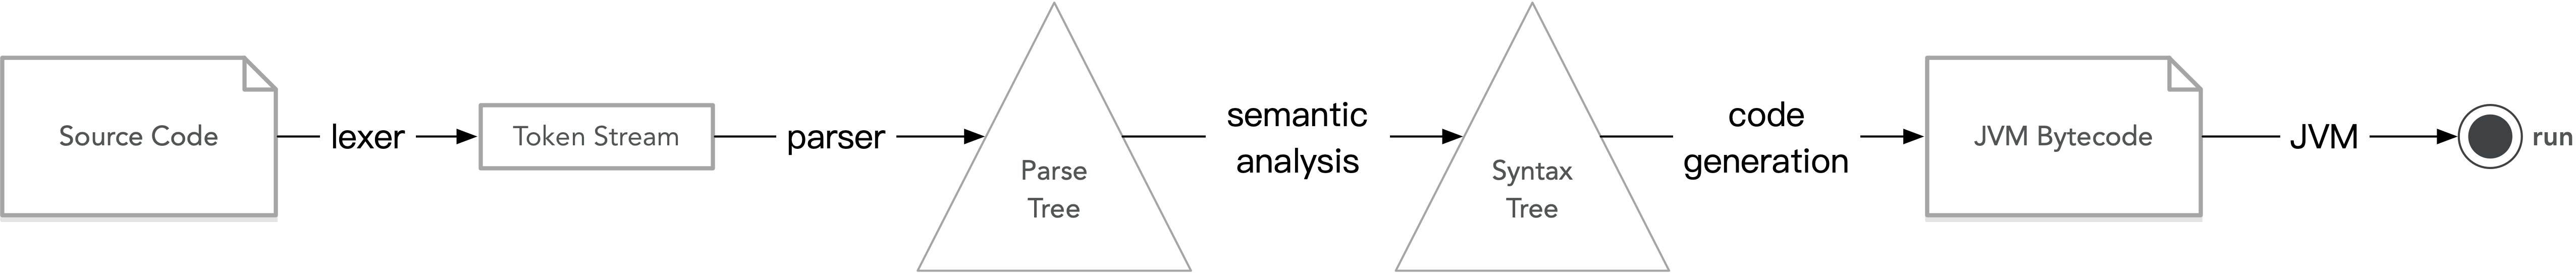
\includegraphics[scale=0.28]{assets/architecture.png}    
    \end{figure}
\end{frame}

\begin{frame}
    \frametitle{Platform \& Dependency}

    \begin{itemize}
        \item[$\blacksquare$] Java 8
        \item[$\blacksquare$] Gradle
        \item[$\blacksquare$] COMMONS-CLI: parse the command line
        \item[$\blacksquare$] ANTLR 4: lexical/syntactic analysis
        \item[$\blacksquare$] ASM: help to generate Java bytecode
    \end{itemize}
\end{frame}

\begin{frame}[fragile]{Code}
    \frametitle{Lexical Analysis}
    With the help of ANTLR, lexical analysis can be easy:
    \begin{block}{Lexical Rules Example}
        \begin{lstlisting}[firstnumber=1, label=glabels, xleftmargin=10pt] 
WHITE_SPACE: [ \t\r\n]+ -> skip;
LINE_COMMENT: '//' ~[\r\n]* -> skip;
CHAR_LITERAL: '\'' [a-zA-Z\\] '\'';
        \end{lstlisting}
    \end{block}
\end{frame}


\begin{frame}[fragile]{Code}
    \frametitle{Syntactic Analysis}
    By ANTLR, we can write the following parsing rules. All the rules are placed in a .g4 file.
    % TODO: code of antlr
    \begin{block}{Parsing Rules Example}
        \begin{lstlisting}[firstnumber=1, label=glabels, xleftmargin=10pt] 
namespaceDefinition:
    NAMESPACE_SYMBOL IDENTIFIER LEFT_CURLY_BRACE codeContent+ RIGHT_CURLY_BRACE;

        \end{lstlisting}
    \end{block}
   \textbf{Note} : ANTLR doesn't support left-recursive, we have to solve it manually.
\end{frame}


\begin{frame}
    \frametitle{Syntactic Analysis}
    Result of Syntactic Analysis:
    \begin{figure}[h]
        \centering
        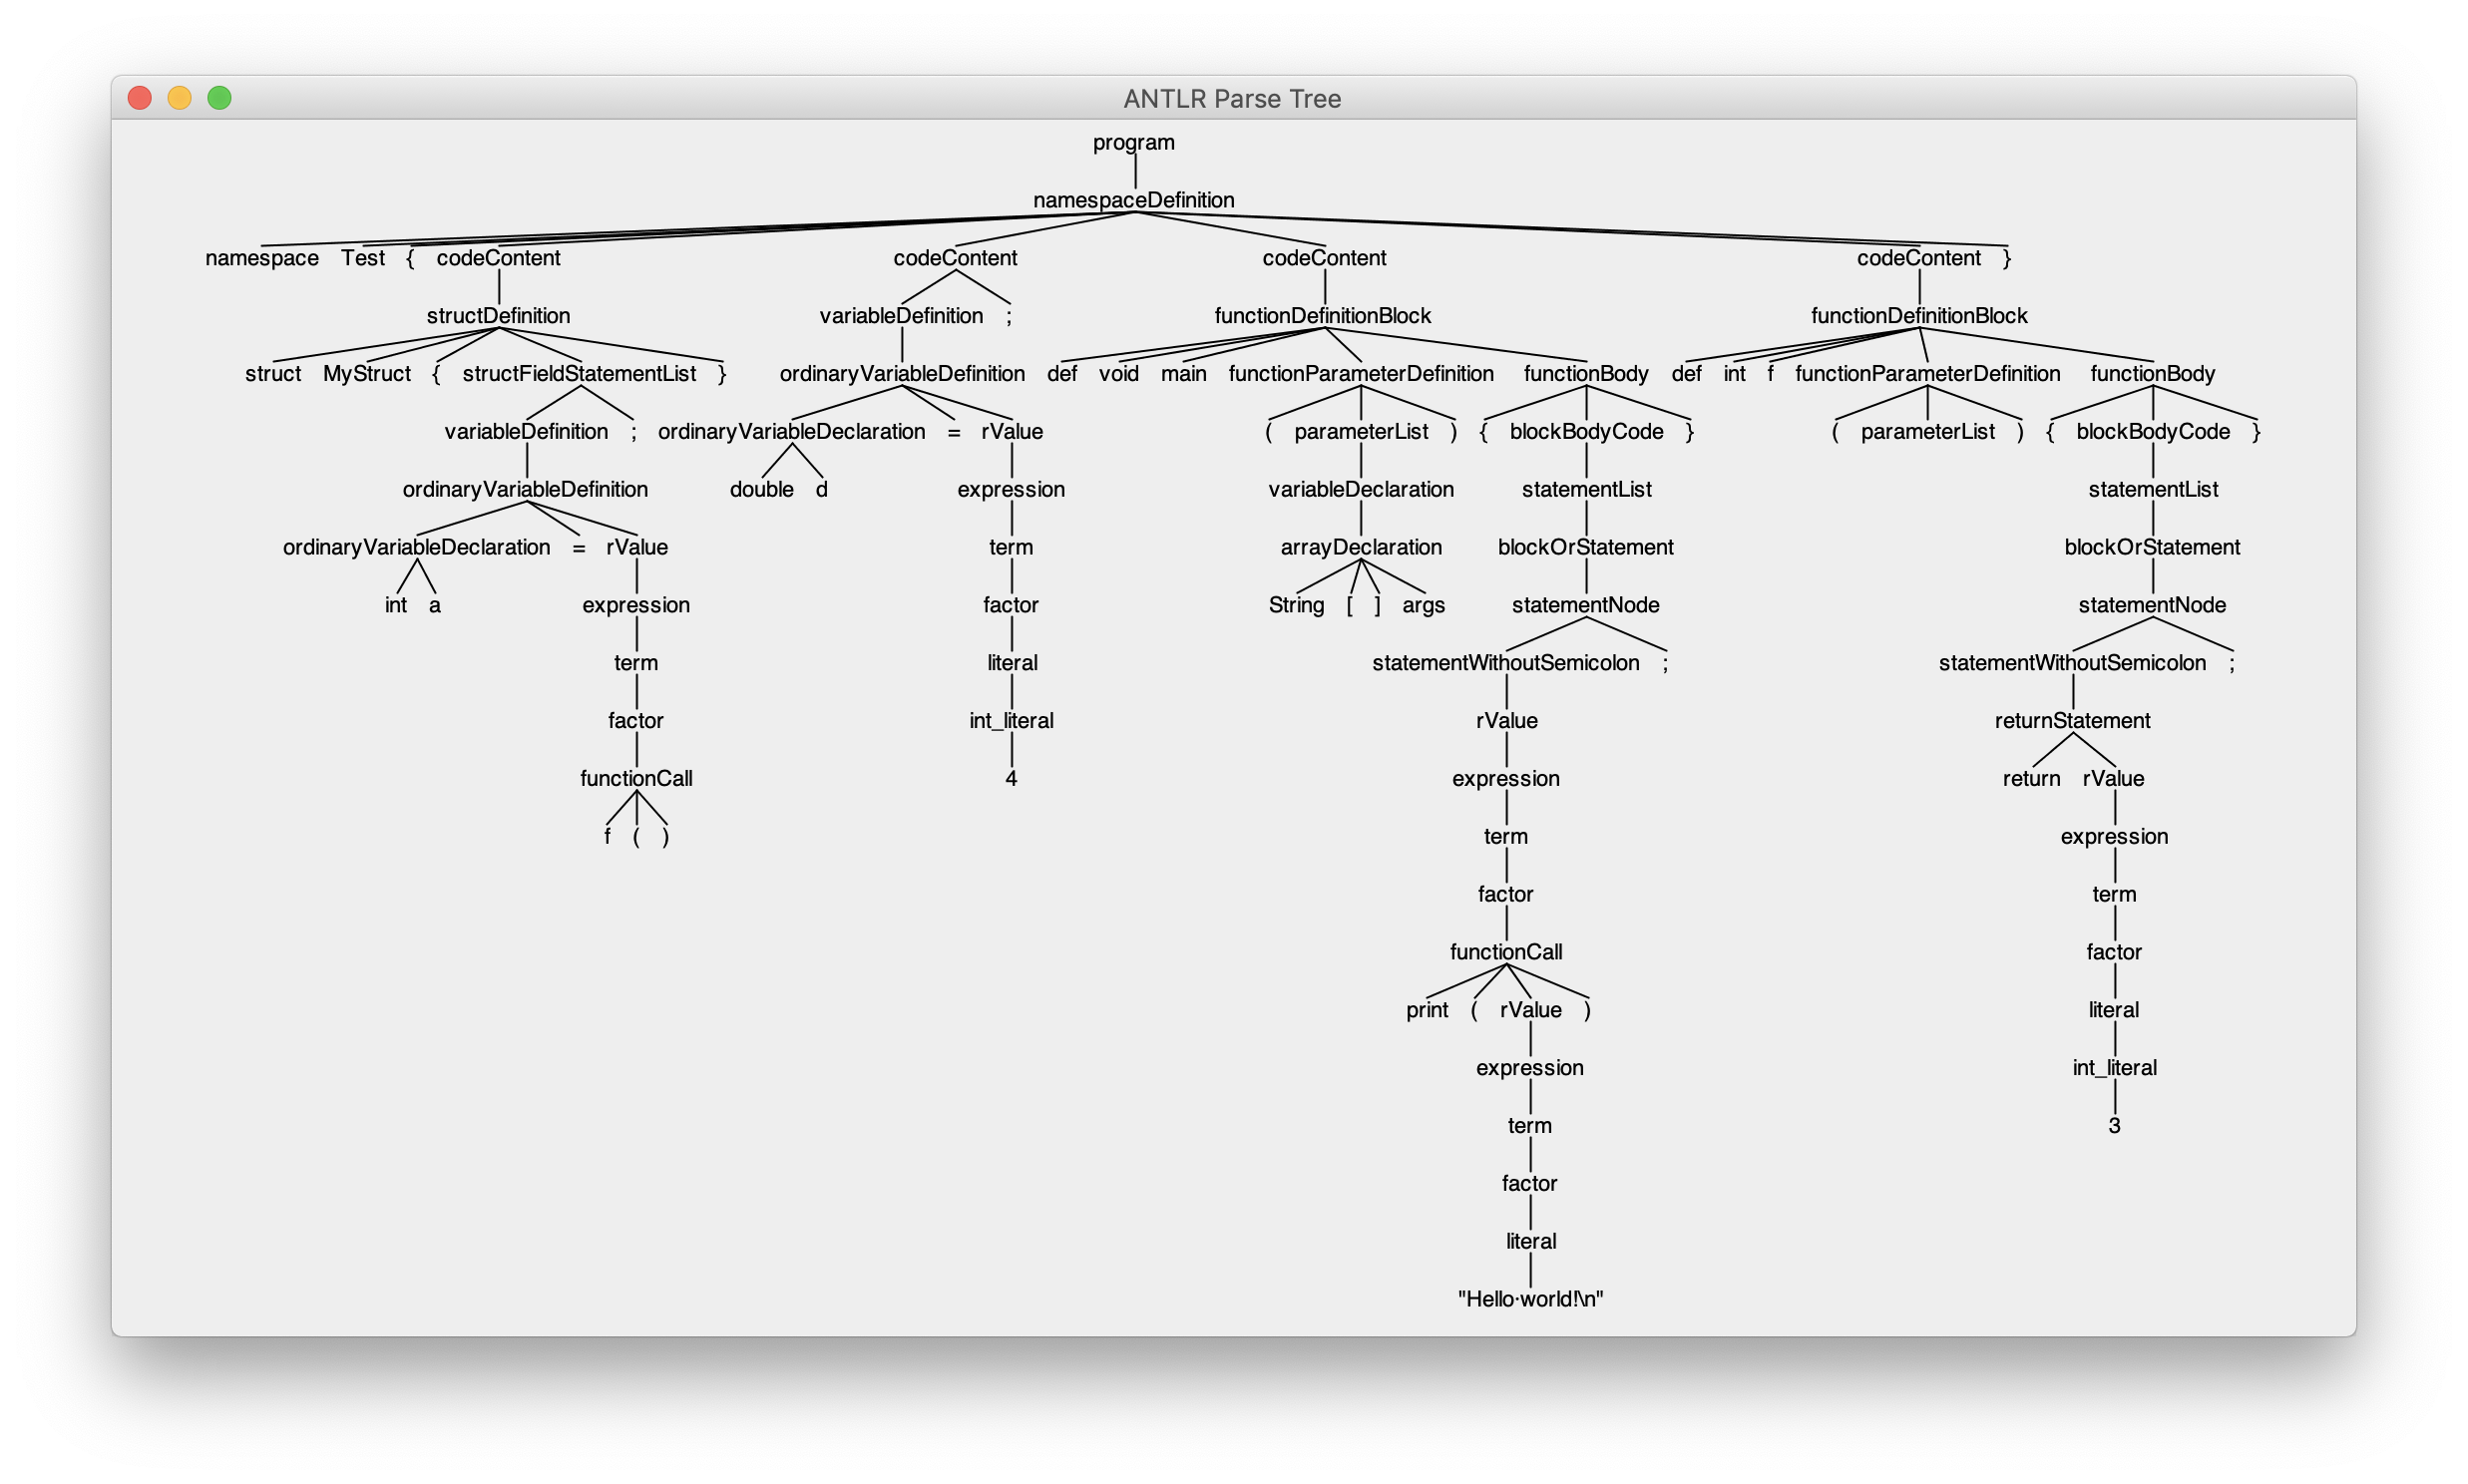
\includegraphics[scale=0.27]{assets/ParseTree.png}
    \end{figure}
\end{frame}

\begin{frame}
    \frametitle{Semantic Analysis}
    Syntax Tree:
    \begin{figure}[h]
        \centering
        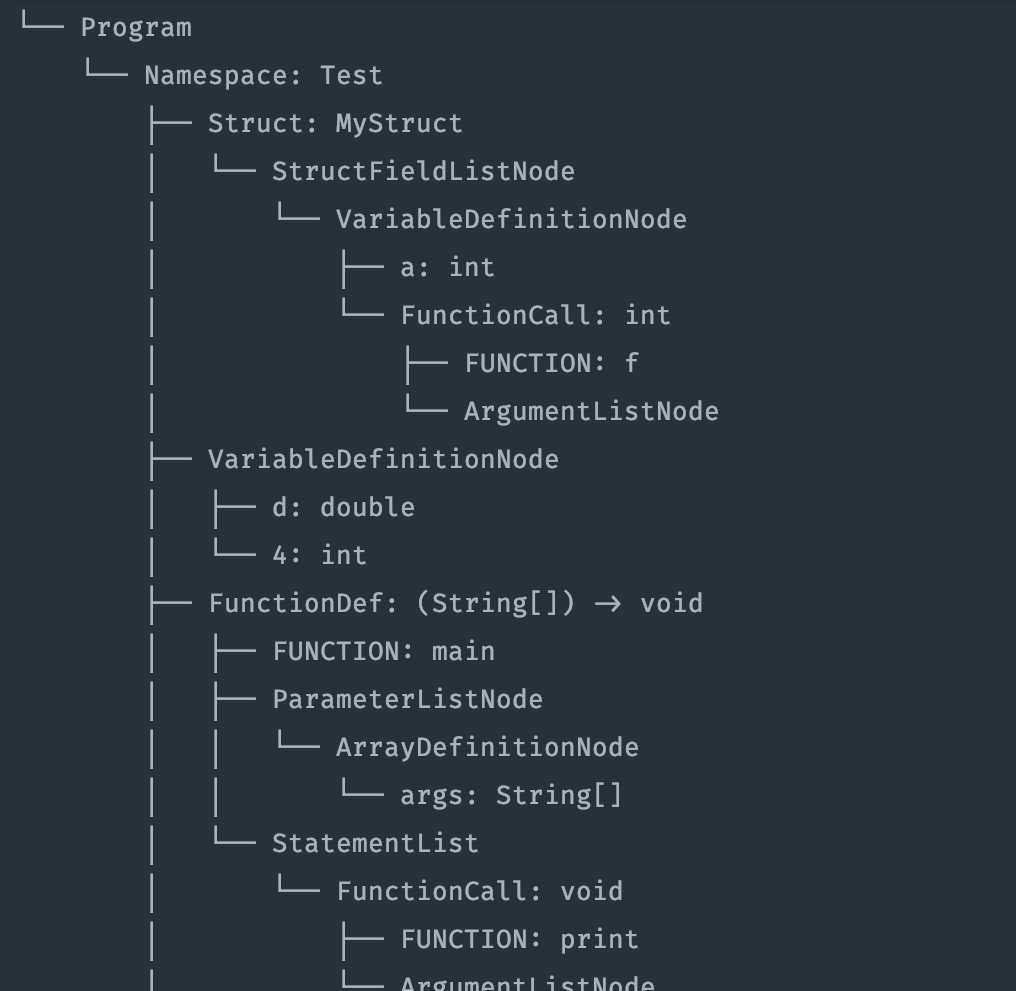
\includegraphics[scale=0.4]{assets/AST.png}
    \end{figure}
\end{frame}

\begin{frame}
    \frametitle{Code Generation}
    \begin{itemize}
        \item[$\blacksquare$] Map from language to JVM inner structure:
    \end{itemize}
    \centering
    \begin{tabular}{|c|c|} \hline
        Structure in this language & Corresponding structure in JVM  \\ \hline
        Namespace & Class \\ \hline
        Struct & Inner class\\ \hline
        Fields in Struct & Fields in inner class\\ \hline
        Variable declared in namespace & Static fields in class\\ \hline
        function & Static method in class \\ \hline
        other & Same as JVM \\ \hline
    \end{tabular}
\end{frame}

\begin{frame}
    \frametitle{Code Generation}
        \begin{itemize}
        \item[$\blacksquare$] Equivalent code between this language and Java:
    \end{itemize}
    \begin{figure}[h]
        \centering
        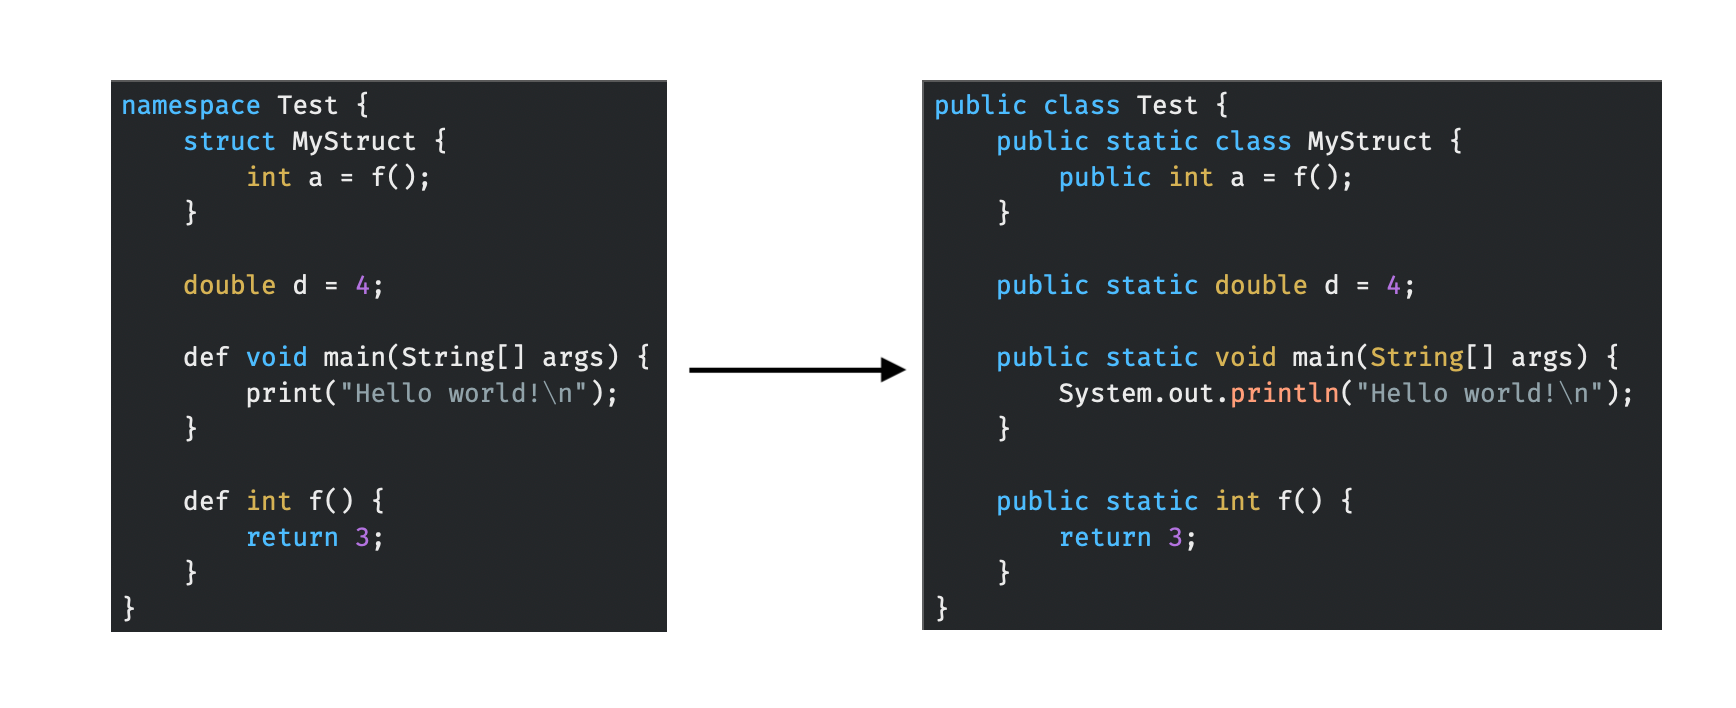
\includegraphics[scale=0.2]{assets/codeConvert.png}
    \end{figure}
\end{frame}

\begin{frame}
    \frametitle{Code Generation}
        \begin{itemize}
        \item[$\blacksquare$] Format of JVM .class file
    \end{itemize}
    \begin{figure}[h]
        \centering
        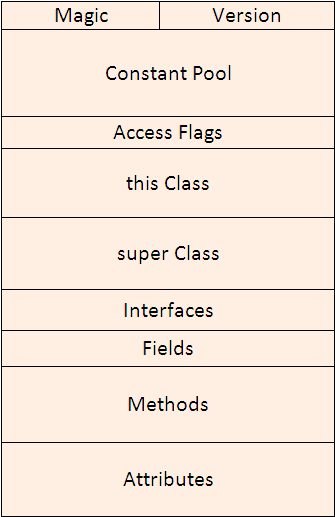
\includegraphics[scale=0.35]{assets/java-class-file-internal-structure.png}
    \end{figure}
\end{frame}

\begin{frame}
    \frametitle{Code Generation}
    \begin{itemize}
        \item[$\blacksquare$] JVM is a stack machine
        \item[$\blacksquare$] JVM assembly language is a kind of P-Code
    \end{itemize}
    \begin{figure}[h]
        \centering
        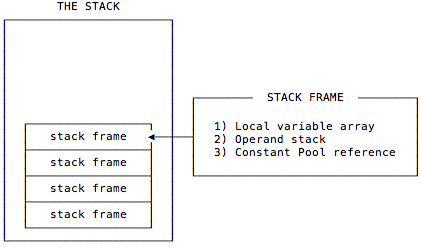
\includegraphics[scale=0.5]{assets/JVM-stack.png}
    \end{figure}
\end{frame}

\begin{frame}[fragile]{Code}
    \frametitle{Code Generation}
    \begin{block}{Pseudocode of for-loop}
        \begin{lstlisting}[firstnumber=1, label=glabels, xleftmargin=10pt] 
for (initStatements; condition; stepStatements) { }
        \end{lstlisting}
    \end{block}
    
    \begin{block}{JVM assembly code of for-loop}
        \begin{lstlisting}[firstnumber=1, label=glabels, xleftmargin=10pt] 
   //do initStatements
loop_label:
    //push condition
    ifeq end_label
    //BlockCode
continue_label:    
    //stepStatements
    goto loop_label
end_label:
        \end{lstlisting}
    \end{block}
\end{frame}

\begin{frame}
    \frametitle{Contributions}
    \begin{itemize}
        \item[$\blacksquare$] Jiawei Chen \\
        lexical analysis (part), semantic analysis, code generation (part), test
        \item[$\blacksquare$] Zhetuo Qi \\
        lexical analysis (part), syntactic analysis, code generation (part)
    \end{itemize}
\end{frame}

\end{document}
